%%% use twocolumn and 10pt options with the asme2ej format
\documentclass[twocolumn,10pt]{asme2ej}

\usepackage{epsfig} %% for loading postscript figures

%% The class has several options
%  onecolumn/twocolumn - format for one or two columns per page
%  10pt/11pt/12pt - use 10, 11, or 12 point font
%  oneside/twoside - format for oneside/twosided printing
%  final/draft - format for final/draft copy
%  cleanfoot - take out copyright info in footer leave page number
%  cleanhead - take out the conference banner on the title page
%  titlepage/notitlepage - put in titlepage or leave out titlepage
%  
%% The default is oneside, onecolumn, 10pt, final

\usepackage{textcomp}
\usepackage{ifthen}
\usepackage[absolute]{textpos}

% Header/Footer
\usepackage{fancyhdr}
\pagestyle{fancy}
\renewcommand{\headrulewidth}{0pt} %gets rid of default line
\lhead{}
\chead{}
\rhead{}
\lfoot{}
\cfoot{\thepage}
\rfoot{Copyright \textcopyright\hspace{1pt} 2015 by The Cooper Union}

\title{DEVELOPMENT OF A CURVED LAYER CARBON FIBER REINFORCED PLASTIC 3D PRINTER}

%%% first author
\author{Peter A. Ascoli
    \affiliation{
	The Cooper Union\\
	New York, NY, USA
    }	
}

%%% second author
\author{Jacqueline G. Song
    \affiliation{
    The Cooper Union\\
	New York, NY, USA
    }
}

%%% third author
%%% remove the following entry for single author papers
%%% add more entries for additional authors
\author{
    \affiliation{ \vspace{-1in}
    }
}

%%%%%%%%%%%%%%%%%%%%%%%%%%%%%%%%%%%%%%%%%%%%%%%%%%%%%%%%%%%%%%%%%%%%%%
\begin{document}

% In top right hand corner, in bold, insert:
%ME 164 Capstone Senior ME Design
%
%The Cooper Union Spring 2015
test
\maketitle

%{\let\newpage\relax\maketitle}   

%%%%%%%%%%%%%%%%%%%%%%%%%%%%%%%%%%%%%%%%%%%%%%%%%%%%%%%%%%%%%%%%%%%%%%
\section*{ABSTRACT}

%%% ABSTRACT %%%

Current desktop 3D printers use FDM (Fused Deposition Modeling) to build parts out of flat layers of extruded thermoplastics. The printed parts have poor mechanical properties because of the low strength of thermoplastics and because the flat layer geometry limits inter-layer adhesion in thin areas. A curved-layer CFRP (Carbon Fiber Reinforced Polymer) 3D printer was developed to solve those two issues. With curved layers, the carbon fiber may be oriented to best suit the applied loading on any given part, and the layers may be designed for greater inter-layer adhesion. An FDM-compatible ABS-matrix CFRP filament was developed by dipping a carbon fiber tow in an ABS-Acetone solution and was shown to have promising mechanical properties, comparable to aluminum. A custom FDM extruder was designed and fabricated for mounting to an available FANUC LR Mate 200iC industrial robot arm, which provides the six degrees of freedom needed to print curved layers. Control electronics, in the form of the FANUC robot system and open-source Megatronics 3D printer microcontroller board, were implemented and programmed to generate a toolpath for a sample specimen and operate the extruder hardware during printing. Finally, a composite-specific finite element analysis predicted the strength of the printed CFRP sample part to be twice that of ABS with stiffness on the same order as and aluminum part of the same geometry.

%%%%%%%%%%%%%%%%%%%%%%%%%%%%%%%%%%%%%%%%%%%%%%%%%%%%%%%%%%%%%%%%%%%%%%
\section*{INTRODUCTION}

%%% INTRODUCTION %%%

Early prior research demonstrated the superiority of ceramics for bearings (1, 2) and the existence of elasto- hydrodynamic (ehd) lubricant films at ball and roller contacts (3), the calculation of which is now an accepted part of bearing engineering.  These new concepts are now used in the design of lubrication systems with solid lubricants that operate in much more severe environments than oils and greases (4, 5).  Proprietary computer codes and unique patented bearing configurations for optimizing the performance of bearing/solid-lubricant systems have been developed (6, 7 and 8).  In this way, patented self-contained solid-lubricated all-steel and hybrid-ceramic ball and roller bearings are now available for environments that do not contribute to their lubrication, such as in air or vacuum.

\clearpage
%\rhead{}
%%%%%%%%%%%%%%%%%%%%%%%%%%%%%%%%%%%%%%%%%%%%%%%%%%%%%%%%%%%%%%%%%%%%%%
\section*{NOMENCLATURE}

%%% NOMENCLATURE %%%

\begin{tabbing}

  XXXXXX \= \kill% this line sets tab stop

  $ABS$ \> Acrylonitrile Butadiene Styrene\\
  $PLA$ \> Polylactic Acid\\
  $FDM$ \> Fused Depostion Modeling\\
  $CFRP$ \> Carbon Fiber Reinforced Plastic/Polymer\\
  $FEA$ \> Finite Element Analysis\\
  $FEM$ \> Finite Element Model\\
  
\end{tabbing}



%%%%%%%%%%%%%%%%%%%%%%%%%%%%%%%%%%%%%%%%%%%%%%%%%%%%%%%%%%%%%%%%%%%%%%
\section*{MATERIALS AND METHODS}

%%% MATERIALS AND METHODS %%%


Put materials and methods used here.

\subsection*{Carbon Fiber Filament}

test text\\

\subsection*{Extruder Design}

An extruder end-effector was designed and fabricated for the curved layer carbon fiber 3D printer. The extruder is the mechanism responsible for depositing the CFRP filament, which is accomplished by reeling in the filament, heating, and printing it. For mounting to the FANUC robot, the extruder's prime design constraints were to includes attachment fixtures for connecting to the robot's Schunk pneumatic gripper and use geometries and materials that minimize torque on the gripper jaws. The designed extruder uses RepRap 3D printing hardware and custom components (machined aluminum and laser-cut acrylic). To drive the filament into the heating chamber, a notched screw, which rests on two bearings, receives a 3:1 step-up in torque from a stepper motor. A bearing for filament counterpressure is mounted between an adjacent set of carrier plates, which can be translated to accomodate filament sizes ranging from 1.75 to 3 mm. Figure~\ref{fig:extruder-side-profile} shows an image of the fabricated extruder, which was designed in SolidWorks, pulling and and printing filament.

%\begin{figure}[htp]
%\centering
%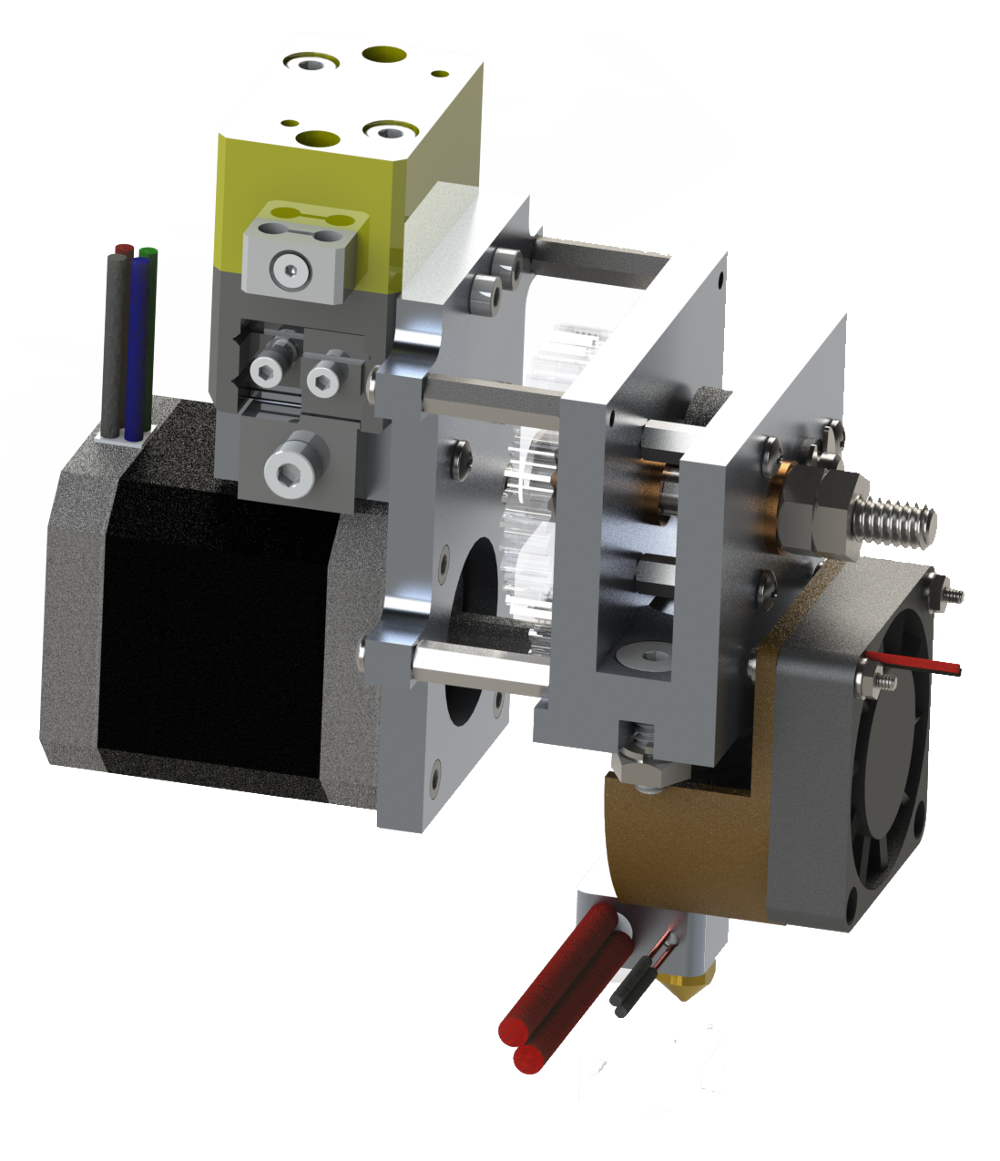
\includegraphics[width=0.8\linewidth]{./figures/extruder-iso}
%\caption{A SolidWorks rendering of the extruder.}
%\label{fig:extruder-iso}
%\end{figure}

\begin{figure}[htp]
\centering
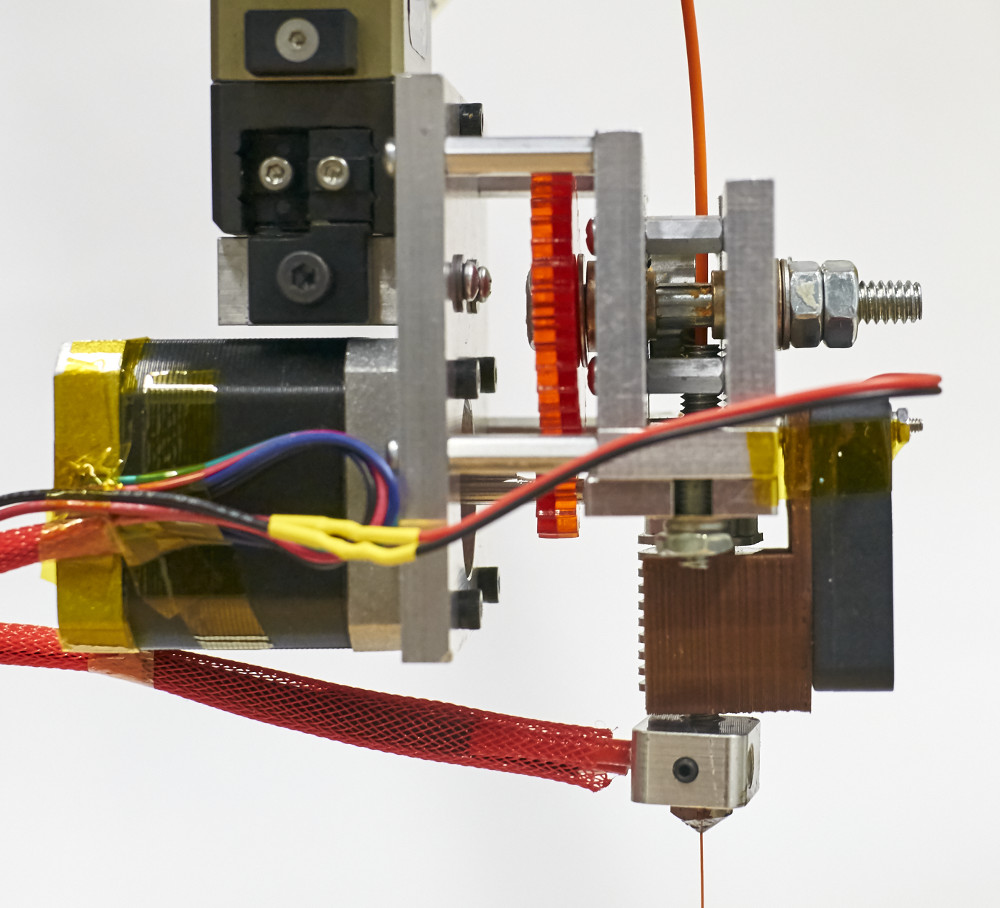
\includegraphics[width=0.8\linewidth]{./figures/extruder-side-profile}
\caption{A SolidWorks rendering of the extruder.}
\label{fig:extruder-side-profile}
\end{figure}

%test text\\

\subsection*{Finite Element Analysis}

ANSYS Composite PrepPost (ACP) finite element analysis software was used to predict the mechanical properties and failure behavior of the bridge specimen. ACP utilizes orthopic shell elements, ply thickness assignments, oriented element sets, and stackup configurations to model and analyze fiberous, composite structures of multiple layers. A surface representation of the bridge specimen, shown in Figure~\ref{fig:fea-bridge-speciment}, was modeled in SolidWorks and imported in ACP. Material properties for ABS and carbon fiber were used in their respective directions to define the orthotropic elements.

Various failure criteria, such as Puck or Tsai-Wu failure theories, can be utilized in ACP to predict failure modes and critical layers given the applied loads and boundary conditions \cite{ACP-manual}. Puck's failure criterion, a phenomenological failure behavior for uni-directional (UD) CFRPs \cite{Puck-Stuttgard,Puck-NASA}, was applied to this model under the loading conditions desribed in the introduction. This mimics the printing condition where all printed CFRP strands are extruded lengthwise so that the carbon fibers react most of the tesile bending stresses caused by compression of the part ends. Figure~\ref{fig:fea-acp-asme} shows the ACP representation of the model, which utilizes a layer thickness 0.4 mm (the extruder end-effector nozzle outlet diameter) to achieve a desired part thickness of 3.175 m.

\begin{figure}[htp]
\centering
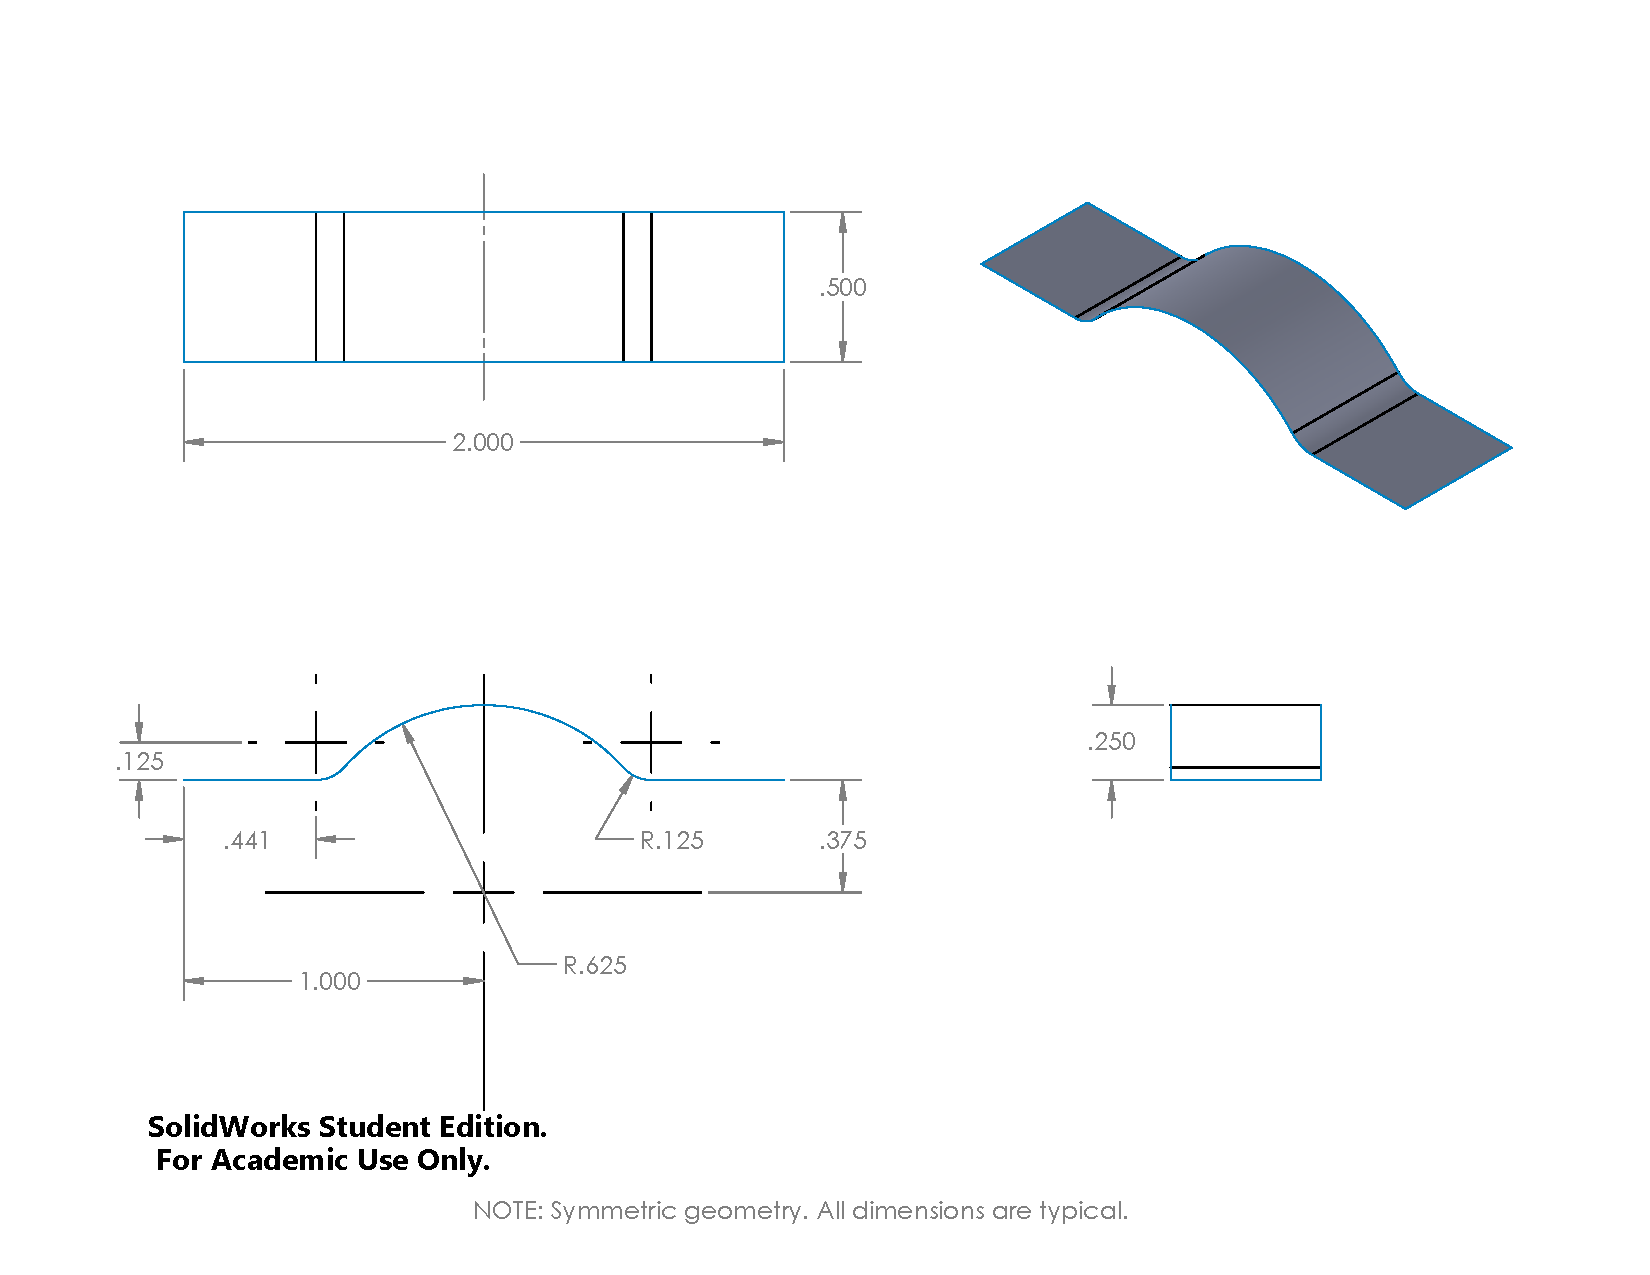
\includegraphics[width=0.8\linewidth]{./figures/fea/fea-surface-geometry}
\caption{The surface geometry used in ACP.}
\label{fig:fea-bridge-speciment}
\end{figure}

\begin{figure}[htp]
\centering
\includegraphics[width=0.8\linewidth]{./figures/fea/fea-acp-asme}
\caption{ACP FEM showing fiber direction and layers.}
\label{fig:fea-acp-asme}
\end{figure}

%test text. test citations \cite{Puck-Stuttgard,Puck-NASA}.\\

\subsection*{Print Controls}

Typical FDM 3D printers, including industrial, home, and do-it-yourself printers, use a Cartesian-style gantry system with 3 degrees of freedom. Such printers can achieve some degree of curved-layer printing, but the fixed print head attitude limits the curved-layer geometries to those accessible from one approach angle. To remove this limitation, a 6-degree-of-freedom FANUC LR Mate 200iC robotic arm was used for this project. The robot provides a similar resolution and repeatibility to other FDM printers, with a somewhat larger build envelope, making it a good candidate to become an FDM printer platform. Some of the remaining elements of the printer control system were chosen from existing open-source hardware and software from the RepRap community, while others were chosen from FANUC products.

Figure~\ref{fig:sys-overview} gives a schematic overview of the mechanical, hardware, and software components that make up the curved-layer 3D printer system. The robot arm is the mechanical platform for the 3D printer. The custom extruder is fitted to the end of the robot arm and acts as a printing end effector. The motion of the robot arm is controlled by the robot controller, which is programmed by writing TP programs via the controller teach pendant. The extruder hardware, including the heater cartridge, cooling fan, and extrusion motor are controlled by an open-source Megatronics board loaded with the (also open-source) Marlin firmware. 

\begin{figure}[t]
    \centering
    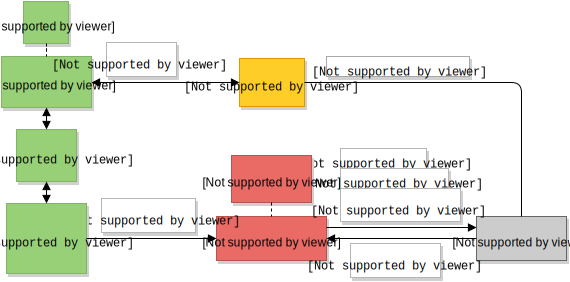
\includegraphics[width=.8\linewidth]{figures/diagrams/system overview}
    \caption{Overview of the 3D printer controls.}
    \label{fig:sys-overview}
\end{figure}

\subsection*{FANUC Setup}

test text\\


%%%%%%%%%%%%%%%%%%%%%%%%%%%%%%%%%%%%%%%%%%%%%%%%%%%%%%%%%%%%%%%%%%%%%%
\section*{RESULTS}

%%% RESULTS %%%

Put results here.

%%%%%%%%%%%%%%%%%%%%%%%%%%%%%%%%%%%%%%%%%%%%%%%%%%%%%%%%%%%%%%%%%%%%%%
\section*{DISCUSSION}

%%% DISCUSSION %%%

Put discussion here.

%%%%%%%%%%%%%%%%%%%%%%%%%%%%%%%%%%%%%%%%%%%%%%%%%%%%%%%%%%%%%%%%%%%%%%
\section*{ACKNOWLEDGEMENTS}

%%% ACKNOWLEDGEMENTS %%%

Put acknowledgements here.

%%%%%%%%%%%%%%%%%%%%%%%%%%%%%%%%%%%%%%%%%%%%%%%%%%%%%%%%%%%%%%%%%%%%%%
\section*{REFERENCES}

%insert bibtex file

\end{document}
